\documentclass[12pt,english]{article}
\usepackage[a4paper,bindingoffset=0.2in,%
            left=0.4in,right=1in,top=1in,bottom=1in,%
            footskip=.25in]{geometry}
\usepackage{amsmath}
\usepackage{amssymb}
\usepackage{graphicx}
\usepackage{hyperref}
\usepackage{listings}
\usepackage{color}

\definecolor{dkgreen}{rgb}{0,0.6,0}
\definecolor{gray}{rgb}{0.5,0.5,0.5}
\definecolor{mauve}{rgb}{0.58,0,0.82}

\lstset{frame=tb,
  language=Matlab,
  aboveskip=3mm,
  belowskip=3mm,
  showstringspaces=false,
  columns=flexible,
  basicstyle={\small\ttfamily},
  numbers=none,
  numberstyle=\tiny\color{gray},
  keywordstyle=\color{blue},
  commentstyle=\color{dkgreen},
  stringstyle=\color{mauve},
  breaklines=true,
  breakatwhitespace=true,
  tabsize=3
}

\graphicspath{ {./grafice/} }

\title{Solutii Existente}
\date{2021\\ Noiembrie}
\author{Ionescu Alexandru Cristian - 342 B3}

\begin{document}

\maketitle
\newpage

\tableofcontents
\newpage

Majoritatea sistemelor de tip interfon, chiar si cele nou instalate sunt bazate pe o tehnologie numita POTS (Plain Old Telephone Service)

\href{https://www.epanorama.net/documents/telecom/telephone_intercom.html}{Simple schema}

\begin{center}
  \fbox{ 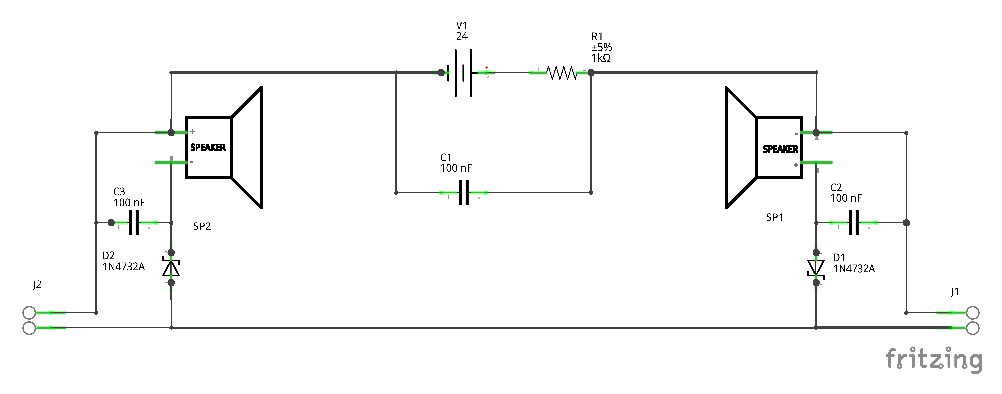
\includegraphics[width=0.8\textwidth]{interfon_schem.pdf}}
\end{center}

\href{https://www.nextiva.com/blog/what-is-pots.html}{Alt articol}

O evolutie normala de la acest sistem, ca si trecerea de la telefonul fix la cel mobil, sunt interfoanele GSM. Acestea au un modul GSM si o agenda telefonica, ce le permite locatarilor sa ofere accesul sau nu in incinta.

\section {Videx UK}

\href{https://www.videxuk.com/system/gsm-intercoms/}{Videx UK}

\section {Interfon GSM}

\href{https://www.a2t.ro/interfoane-videointerfoane/interfon-wireless-gsm-pentru-o-familie.html}{Link}

Interfon wireless GSM pentru o familie si controlere GSM pentru deschidere de porti sau bariere. Foarte util pentru zonele in care nu exista cablaje. Poate deschide o yala, o automatizare sau o bariera. Vorbesti cu vizitatorii direct de pe telefonul tau mobil. Functioneaza pe reteaua oricarui operator de telefonie mobila 2G.

\section {Hikvision DS-KV8413-WME1}

\href{https://www.a2t.ro/videointerfon-wireless/videointerfon-full-hd-4-familii-control-acces-aplicat-tcp-ip-hikvision-ds-kv8413-wme1-s.html}{Link}

\href{https://www.hikvision.com/content/dam/hikvision/products/S000000001/S000000083/S000000129/S000000131/OFR000170/M000048926/User_Manual/UD20207B_Baseline_Video-Intercom-8-Series-Villa-Door-Station_User-Manual_V2.2.3.PDF}{Manual}


Post de exterior, camera 2MP, WiFi Proxi, 4 butoane de apelare, reducere zgomot si ecou, audio bidirectional, BLC, DNR, WDR, IP65, IK08, PoE / 12VDC. Montaj ingropat.

Video-interfon metalic, cu 4 butoane (pentru 4 familii).

\end{document}